% ===========================================================================================================
% TEX file generated by R with the 'knitr' package
%
% DO NOT EDIT THE TEX FILE DIRECTLY
% ===========================================================================================================

\documentclass{report}\usepackage{knitr}

% Captions in floating environments
\usepackage[labelsep=colon,tableposition=top,font=small,margin=5pt,format=hang]{caption}

% For subcaptions in figures
\usepackage{subcaption}

% For sidewaysfigure
%\usepackage{rotfloat}

% For professional looking tables
\usepackage{booktabs} 

%\usepackage{multirow}
%\usepackage{multicol}
%\usepackage{longtable}
%\usepackage{tabularx}

% For underscores that correspond to the encoding
\usepackage[T1]{fontenc}

% For \FloatBarrier
\usepackage[section,below]{placeins}

% Linebreaks in tables
\usepackage{makecell}

% Hyperlinks
\usepackage{hyperref}

% Table of content settings
\setcounter{tocdepth}{2}
\setcounter{secnumdepth}{2}

% Allowed percentages of page a float can use
\renewcommand{\textfraction}{0.05}
\renewcommand{\topfraction}{0.95}
\renewcommand{\bottomfraction}{0.95}
\renewcommand{\floatpagefraction}{0.75}
\setcounter{totalnumber}{5}

% Figure names
\renewcommand{\figurename}{Fig.}

% changes the default name `Bibliography` -> `References'
\renewcommand{\bibname}{References}

\newenvironment{romanpages}{
  \setcounter{page}{1}
  \renewcommand{\thepage}{\roman{page}}}
{\newpage\renewcommand{\thepage}{\arabic{page}}}

% Used for knitr images from Rnw files
\newcommand{\subfloat}[2][default for first parameter: need a sub-caption]{\subcaptionbox{#1}{#2}}

% Typesetting commands
\newcommand{\R}{\textbf{\textsf{R}}}

\IfFileExists{upquote.sty}{\usepackage{upquote}}{}
\begin{document}

% REMINDER: working directory for *chunk headers* and *knitr options* is always directory of **root** file...

% Chunk names must be unique, considering any and all chunks from children files



% ===========================================================================================================
% Cover
% ===========================================================================================================

\title{Thesis Template using R and knitr}
\author{Alexis Sard\'a-Espinosa}
\date{\today}

\maketitle

% ===========================================================================================================
% Front matter
% ===========================================================================================================

\pagenumbering{Roman}

\chapter*{Dedication}
To me

\chapter*{Abstract}
Abstract goes here

\chapter*{Declaration}
I declare that..

\chapter*{Acknowledgements}
I want to thank...

\tableofcontents

\listoffigures

\listoftables

% ===========================================================================================================
% Main matter
% ===========================================================================================================

\cleardoublepage
\pagenumbering{arabic}

\chapter{Introduction}
\label{ch:introduction}

\section{Introduction}
\label{sec:introduction}

I did my thesis in \R{}, and it took me a while to get everything working the way I wanted. The example here is a skeleton that could serve as a starting point to write not only theses, but any kind of document using \LaTeX{} and \R{}.

The main files have a \texttt{Rnw} extension and are transformed into \texttt{tex} files by using the \texttt{knitr} package.\footnote{\url{http://yihui.name/knitr/}} However, anything that doesn't depend on \R{} can be written directly in \texttt{tex} files, making it flexible.

I didn't put too much effort into the layout shown here, it is only meant to serve as a starting point with some examples. Other templates can also be used.


\chapter{Examples}
\label{ch:examples}


\section{Basics}
\label{sec:basics}





Using a random forest with the Chess dataset and OOB error estimate, best value of \texttt{mtry} was 13 with an accuracy of 0.995.

Try compiling the thesis with parallel support to see the difference in run time.




\section{Figures}
\label{sec:figures}



\graphicspath{Examples/Figs/}

See Fig.~\ref{fig:iris-histograms} for an example of a single plot.

\begin{knitrout}
\definecolor{shadecolor}{rgb}{0.969, 0.969, 0.969}\color{fgcolor}\begin{figure}[htpb]

{\centering 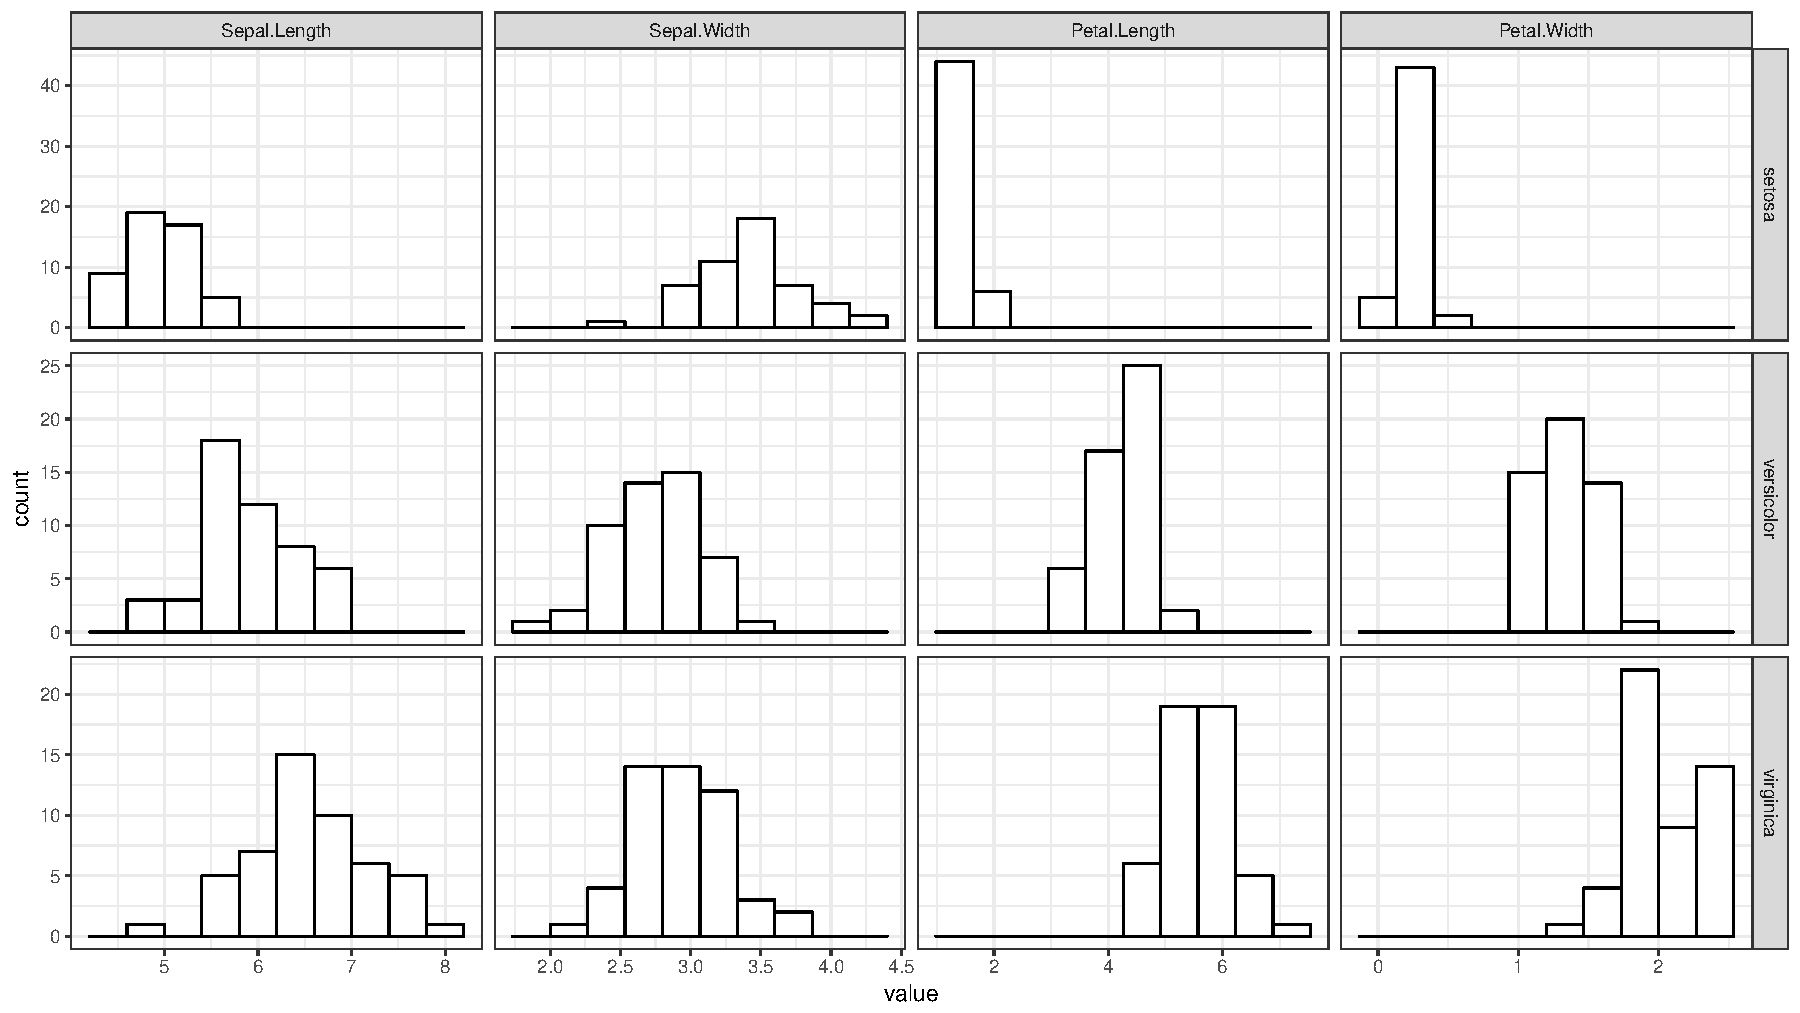
\includegraphics[width=\linewidth]{Examples/Figs/iris-histograms-1} 

}

\caption[Histograms for the iris dataset]{Histograms for the iris dataset. Look at the list of figures to see difference between short and long captions.}\label{fig:iris-histograms}
\end{figure}


\end{knitrout}

See Fig.~\ref{fig:mtcars-subplots} for an example of two plots: Fig.~\ref{fig:mtcars-subplots1} and Fig.~\ref{fig:mtcars-subplots2}.

\begin{knitrout}
\definecolor{shadecolor}{rgb}{0.969, 0.969, 0.969}\color{fgcolor}\begin{figure}[htpb]

{\centering \subfloat[MPG vs HP\label{fig:mtcars-subplots1}]{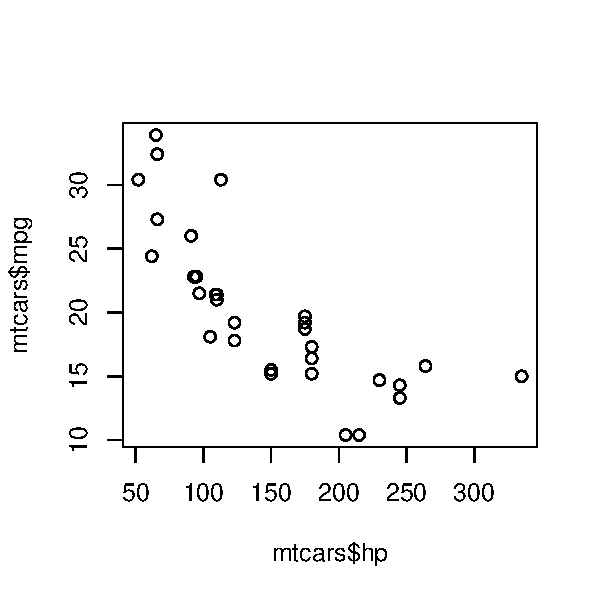
\includegraphics[width=0.45\linewidth]{Examples/Figs/mtcars-subplots-1} }
\subfloat[MPG vs Weight\label{fig:mtcars-subplots2}]{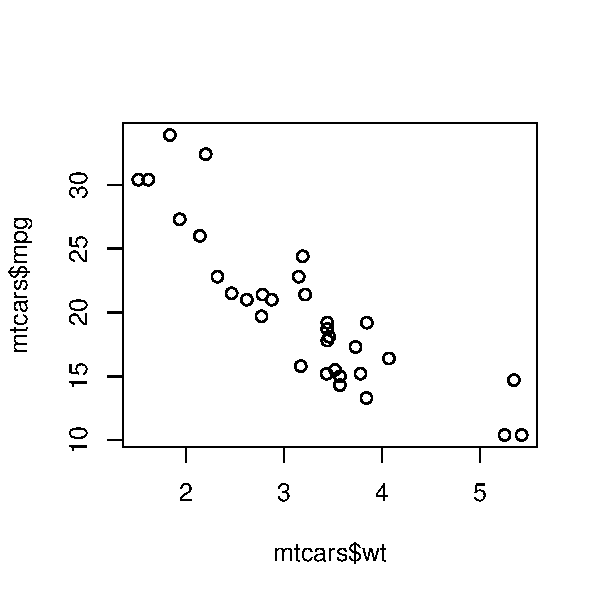
\includegraphics[width=0.45\linewidth]{Examples/Figs/mtcars-subplots-2} }

}

\caption[Plots using \texttt{mtcars} dataset]{Plots using \texttt{mtcars} dataset.}\label{fig:mtcars-subplots}
\end{figure}


\end{knitrout}




\section{Tables}
\label{sec:tables}

% latex table generated in R 3.2.4 by xtable 1.8-2 package
% Sun Mar 13 14:41:42 2016
\begin{table}[htbp]
\centering
\caption[First rows of the CO2 dataset]{First rows of the CO2 dataset. Look at the list of tables to see the difference between short and long table caption.} 
\label{tab:co2_head}
\begin{tabular}{lccccc}
  \toprule
 & Plant & Type & Treatment & conc & uptake \\ 
  \midrule
1 & Qn1 & Quebec & nonchilled & 95.00 & 16.00 \\ 
  2 & Qn1 & Quebec & nonchilled & 175.00 & 30.40 \\ 
  3 & Qn1 & Quebec & nonchilled & 250.00 & 34.80 \\ 
  4 & Qn1 & Quebec & nonchilled & 350.00 & 37.20 \\ 
  5 & Qn1 & Quebec & nonchilled & 500.00 & 35.30 \\ 
  6 & Qn1 & Quebec & nonchilled & 675.00 & 39.20 \\ 
   \bottomrule
\end{tabular}
\end{table}




% ===========================================================================================================
% Bibliography
% ===========================================================================================================

\bibliographystyle{plainnat}
\nocite{*}
\bibliography{References}
\cleardoublepage

% ===========================================================================================================
% Appendices
% ===========================================================================================================

\appendix

\chapter{First Appendix}

\end{document}
